\documentclass[11pt,a4paper]{scrartcl}
\usepackage[utf8]{inputenc}
\usepackage[english]{babel}
\usepackage{amsmath}
\usepackage{amsfonts}
\usepackage{amssymb}
\usepackage{graphicx}
\usepackage{hyperref}
\usepackage[cm]{fullpage}
\usepackage{tablefootnote}


  
\author{Diego Ballesteros, Trajche Kralev, Tribhuvanesh Orekondy}
\title{DJ Byg Data}
\subtitle{The scalable information platform for song lyrics}
\date{\today}

\begin{document}
  \maketitle
  \section{Introduction}

	  During the first part of this project created a small scale implementation
	  for our system where we analyzed a dataset of 10,000 songs. Our main aim
	  being:
	  
	  \emph{The development of a system that can categorize songs by different
	  genres by solely analyzing the song lyrics.}
	
	  Now during the second step we will expand our dataset to a few hundred thousand
	  songs and we will be creating a scalable implementation of the system.

		In this report we first look at the data model and the modeling decisions
		we made concerning the large scale implementation, we then talk about the
   	system architecture and tools which we have used, and finally we discuss the
   	results of the implementation and how it compares to the first part of the
   	project.

  \section{Data model}
    \subsection{Introduction}

    One of the main limitations encountered during the small scale implementation
    we encountered during the first iteration of the project is that the
    intersection of the songs that have lyrics available in the musiXmatch
    dataset and at least one valid genre within the Last.fm tags is too small to
    produce significant results, in the small scale out of the $10000$ subset only
    $1400$ were left after filtering them with this criteria.
    
    In order to overcome this limitation, it was decided that for the scalable
    implementation, these tags would be ignored as a criteria for filtering or
    deciding a cluster's genre and instead they would be used only for quality
    metrics. This allowed the use of the full set of songs with lyrics in the
    million song dataset, the number of songs in this set is $237662$, i.e. 
    $23.7\%$ of the million song dataset.
    
    \subsection{Models}
    \subsubsection{Genre discovery}
    
    From the experience of the proof of concept, it was concluded that the
    clustering approach is adequate for the task at hand. And it is expected
    that with a larger amount of data it will be possible to distinguish
    more clearly the clusters and their genre correspondence. Therefore
    for the scalable implementation the clusters will be kept as the information
    model produced from the data.
    
    This allows for great scalability, because these clusters can be computed
    with a single pass on the data, in addition to the passes done to tune
    the parameters of the computation. Moreover, clusters allow for efficient
    updates if is to be received, since the usual K-means algorithms can
    be formulated in a streaming fashion.
    
    Additionally, it is also necessary to keep term frequencies and
    document frequencies in order to allow query points to be assigned
    to clusters and also the updated of these clusters with new data.
    
    \subsubsection{SQL database}
    In this project there exists a fortunate exception to the usual Big Data
    scenarios, the data has been cleaned and structured for academic and
    research purposes beforehand. Therefore, in light the quality of the data,
    it was decided that the approach to be used for the storage of the data would
    be a SQL database, namely a PostgreSQL database deployed on Amazon's RDS
    service.
 
    This option was chosen because of the following reasons:
 
    \begin{itemize}
      \item It reduces the complexity during the query phase which is used to
            compute statistics and quality metrics
      \item It is compatible with the processing model which requires only a
            single pass on the data, and then storage of the result. There
            is no need for scalability for writes.
      \item It can be scaled for read operations, by spawning read copies
            according to the load. This is possible because of the assumption
            that there is not new data often.
    \end{itemize}        
 
    The schema for the data is presented in figure \ref{fig:data_schema}.
 
    \begin{figure}
      \centering
      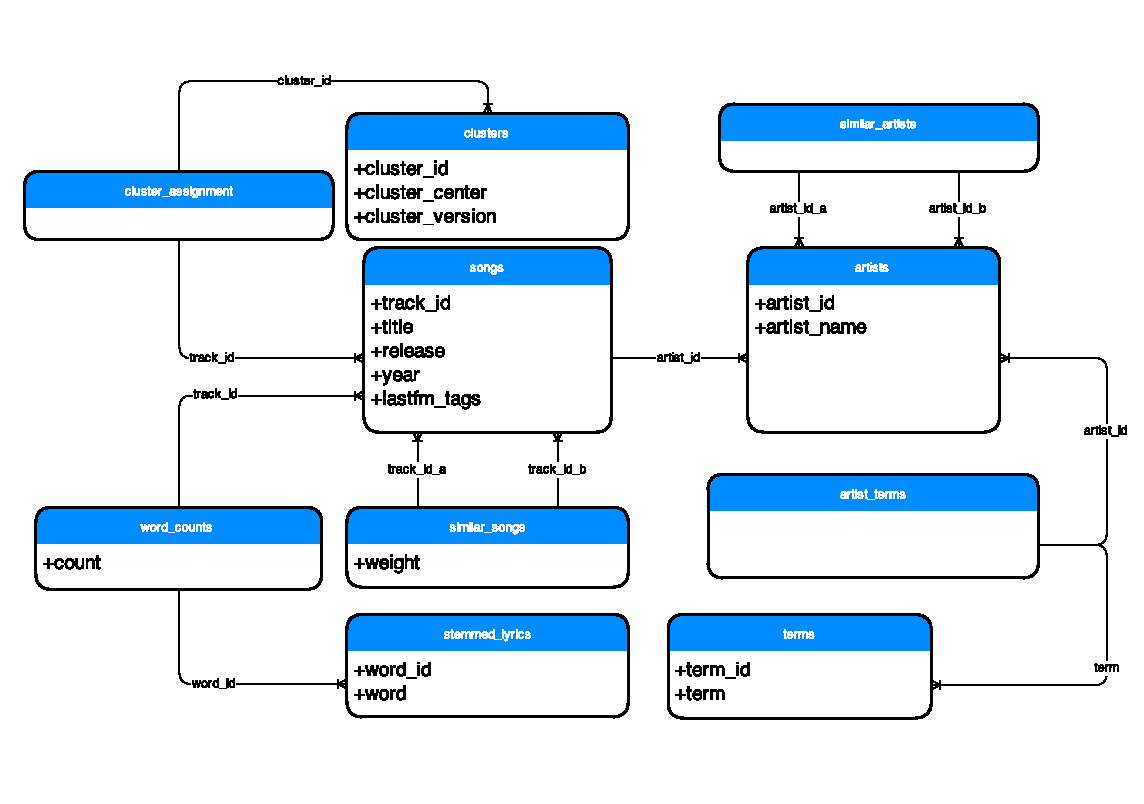
\includegraphics[scale=0.6]{img/database}
      \caption{SQL database schema}
      \label{fig:data_schema}
    \end{figure}        

    \subsection{Preprocessing}
    \subsubsection{Lyrics preprocessing}
    \label{sec:preprocessing}

    For the processing of the data, i.e. clustering the songs based on their
    lyrics content, only the musiXmatch was required. This dataset is available
    as two zip files\footnote{These are provided as test and train dataset for
    academic purposes} where each file contains a single text file and in this
    file each line has the following format:
    
    \emph{track\_id,word\_id:count,word\_id:count,...}
    
    These files were merged and processed in a single machine to produce a file
    with a single 
    \emph{track\_id,word\_id,count} triplet per line. Additionally, the word id
    to stemmed word mapping was extracted from the header of the original files
    and stored in a separate file, it is important to note that this id is simply
    and index from 1 to 5000 which provides an ordering for the words.
    The resulting file with the word frequencies per track has 19M entries and a
    size of 450MB.
    
    The next step in the preprocessing of the lyrics was calculating the
    TF-IDF vectors for each song. Given the size of the input file and the
    natural parallelization of this task, it was decided to implement this
    step using MapReduce in a Hadoop cluster, namely in the AWS EMR service.
    To prepare for this computation, the input file was stored in an S3 bucket
    where it can be accessed by the cluster.
    
    In this case two rounds of MapReduce were necessary to calculate
    the TF-IDF vectors, given that the term frequencies were already available in
    the input file.
    These rounds are summarized in table \ref{tab:mapreduce-tfidf}.
    
    \begin{table}
	    \centering
	    \caption{TF-IDF MapReduce}
	    \begin{tabular}{|c||c||c||c|}
	      \hline
	      Round & Input & Map output & Reduce output \\
	      \hline
	      1 & track\_id,word\_id,count & Key: word\_id &
	      track\_id,word\_id,idf,tf\\
	        &                          & Value: track\_id,count & \\
	      \hline
	      2 & track\_id,word\_id,idf,tf & Key: track\_id & track\_id
	      TF-IDF-vector\\
	        &                           & Value word\_id, idf, tf & \\
	      \hline
      \end{tabular}
      \label{tab:mapreduce-tfidf}
    \end{table}
    
    In the first step, the document frequencies for all terms were calculated. In
    order to do this, the word id was set as the map's output key and then
    it was possible to calculate the document frequencies in the reducers.
    The reducers also computed the TF and IDF values according to equations
    \ref{eq:tf} and \ref{eq:idf} respectively.
    
    \begin{eqnarray}
      \label{eq:tf}
      tf = \sqrt{word\_count}\\
      \label{eq:idf}
      idf = \log{\left(\frac{corpus\_size}{doc\_freq + 1}\right)} + 1
    \end{eqnarray}
    
    In the second step the mapper simply streamed the input data with the track
    id as the key. Therefore it was possible to build the TF-IDF vectors in the
    reducers, using the word ids as the indexes in the vectors.
    Finally, this output was stored back in the S3 bucket for the subsequent
    clustering which will be described later on.
  
	  \subsection{Database preparation}
	
	  In order to fill up the SQL database with the rest of the information, it was
	  necessary to process the individual SQLite files provided with the dataset
	  and create CSV files that can be loaded quickly into the database tables.
	  The source files and the resulting database tables are summarized in table
	  \ref{tab:database_stats}.
	  
	  \begin{table}
	    \centering
	    \caption{Database statistics}
	    \begin{tabular}{|c||c||c||c|}
	    \hline
	    Source & Source size & Target table & \# of records \\
	    \hline
	    track\_metadata.db & 685MB - 1M tracks & songs &
	    237662\tablefootnote{Only songs present in the musiXmatch dataset were
	    kept} \\
	    & & artists & 20521 \\
	    \hline
	    lastfm\_tags.db & 567MB - 8.5M (song, tag) pairs & songs &
	    173730\tablefootnote{This is the number of records with at least one tag}\\
	    \hline
	    artist\_term.db & 133MB - 1M (artist, term) pairs & terms & 6254\\
	    & & artist\_terms & 600570\\
	    \hline
	    lastfm\_similars.db & 3.8GB - 600k songs\tablefootnote{A single row
	    contains all the pairs associated with a song}
	    & similar\_songs & 8866734 \\
	    \hline
	    artist\_similarity.db & 322MB - 2M pairs & similar\_artists & 700608\\
	    \hline
	    \end{tabular}
	    \label{tab:database_stats}
	  \end{table}     
  
  \section{System architecture}
  
  Figure \ref{fig:architecture} presents the different components of the system.
  
  \begin{figure}
    \centering
    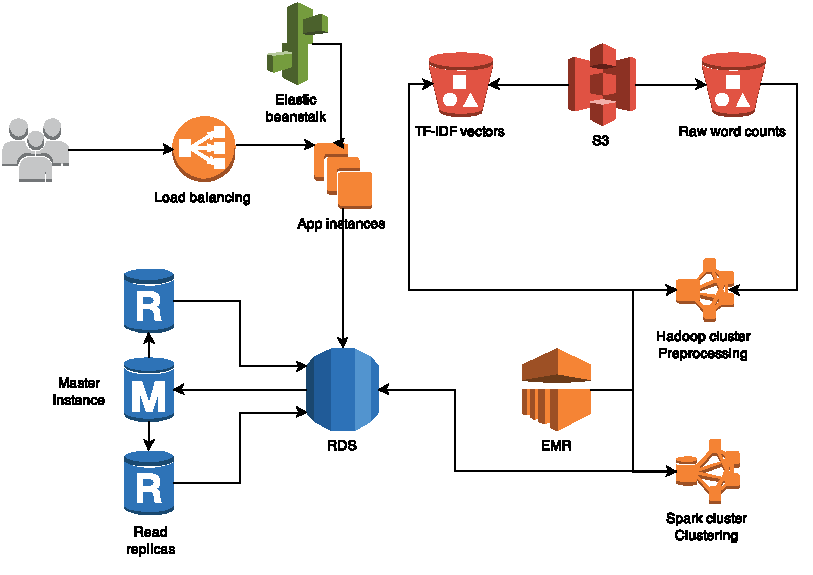
\includegraphics[scale=0.8]{img/architecture}
    \caption{System components}
    \label{fig:architecture}
  \end{figure}          
      
  This system uses different services offered in AWS as building blocks for a
  scalable solution. In the following sections the different components will
  be introduced in more detail.
  
  \subsection{Preprocessing}

  The preprocessing component executes the workflow described in section
  \ref{sec:preprocessing}, the use of EMR and more specifically Hadoop's
  MapReduce provides great flexibility in regards on how big the input is, i.e.
  number of tracks and lyrics, because of the parallel nature of the
  calculation of TF-IDF vectors. Additionally, the use of S3 as a buffer for
  the data guarantees high performance as it is implemented using the Dynamo
  key-value store.
  
  \subsection{Storage}
  
  The RDS service provides also an scalable solution for read-heavy workloads
  as the ones for which the system is being designed, a single pass on the data
  produces the structured entities which are written only once into the system.
  Afterwards, what is expected of the system is to answer different queries from
  multiple users and in this case the use of read replicas allows horizontal
  scalability.
  
  \subsection{Compute}
  
  The computation of clusters from the data is done by reading the resulting
  TF-IDF vectors from the MapReduce's output in S3. 
  
  TODO: Please write how Spark scales with the data here. Probably same argument, that if the data size grows then you just put more machines to do the calculation.
  
  \subsection{Interface}
  
  Finally, the system is exposed to the users via web interface which is deployed
  on AWS ElasticBeanstalk, this makes it possible to spin out EC2 instances on
  demand based on the load which guarantees the horizontal scalability of
  the system. Each of the application server instances holds no state, and simply
  executes the user queries against the database and renders the view, i.e.
  HTML/CSS/JS, with the results.
  
  With this architecture, it is possible to respond to an increasing number of
  users by either deploying a new EC2 instance or a read replica of the
  database. This has no hard limit on the computation side, and only
  would require considerations on the financial cost.
  
  \section{Results}
  %\bibliographystyle{acm}
  %\bibliography{report_1}
\end{document}